\section{Optimal encoding of partial orders\label{sec:Optimal-encoding-problem}}

This section shows the effect of different encoding of partial orders
on the size of the resultant CPOG.

Consider a processing unit that has an accumulator register $A$ and
a general purpose register $B$, and computes four different arithmetic
functions: $(-a)$, $(a+b)$, $(a-b)$, $(-a-b)$. The event domain
contains the following events:

\renewcommand{\labelenumi}{\alph{enumi})}
\begin{enumerate}
\item Load register $A$ from memory;
\item Load register $B$ from memory;
\item Negate value stored in one of the registers;
\item Compute sum $A+B$ and store the result in $A$;
\item Save register $A$ into memory.
\end{enumerate}
The four instructions are described as partial orders of the above
events in Figure~\ref{fig-Four-DAGs-specifying} (we use \emph{Hasse
diagrams}~\cite{1967_birkhoff_} to represent partial orders concisely,
viz. without transitive dependencies). For instance, the second instruction
(computation of $(a+b)$ shown in Figure~\ref{fig-Four-DAGs-specifying}(b))
consists of events $a$ and $b$ happening concurrently (loading of
registers $A$ and $B$), which are followed by event $d$ (addition)
and finally by event $e$ (saving the result).

\begin{figure}[h]
\begin{centering}
\subfloat[$(-a)$]{

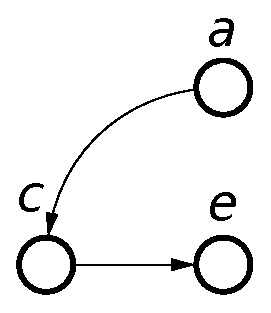
\includegraphics[scale=0.45]{fig/dag_neg}}\hfill{}\hfill{}\hfill{}\subfloat[$(a+b)$]{

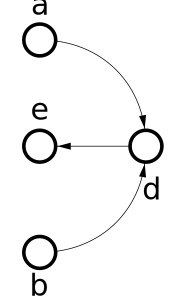
\includegraphics[scale=0.45]{fig/dag_add}}\hfill{}\hfill{}\hfill{}\subfloat[$(a-b)$]{

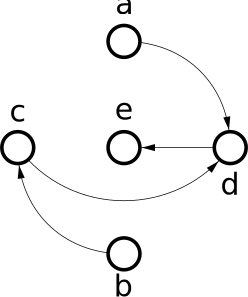
\includegraphics[scale=0.45]{fig/dag_sub}}\hfill{}\hfill{}\hfill{}\hfill{}\subfloat[$(-a-b)$]{

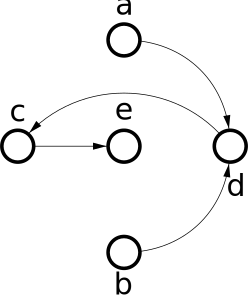
\includegraphics[scale=0.45]{fig/dag_nadd}}
\par\end{centering}

\caption{Partial orders of the instructions\label{fig-Four-DAGs-specifying}}
\end{figure}


Before synthesis of a CPOG $H=(V,\ E,\ X,\ \rho,\ \phi)$ containing
these instructions it is necessary to encode them, i.e. to derive
a set of variables $X=\{x_{1},\ x_{2},\ \dots,\ x_{m}\}$ and a set
of Boolean vectors $\{\psi_{1},\ \psi_{2},\ \dots,\ \psi_{n}\},\ \psi_{k}\in\{1,\ 0\}^{m}$
(opcodes), each of them corresponding to a particular partial order.
Note that $V$ and $E$ can be defined as unions of vertices and arcs
of the given partial orders, $\rho$ as a disjunction of generated
opcodes, and $\phi(z),\ z\in V\cup E$ as a disjunction of opcodes
corresponding to the partial orders containing $z$. Let us examine
several possible encoding schemes to see how a particular scheme affects
the resultant CPOG.

\begin{figure}[th]
\begin{centering}
\subfloat[Binary encoding (00, 01, 10, 11) and projection under opcode 01]{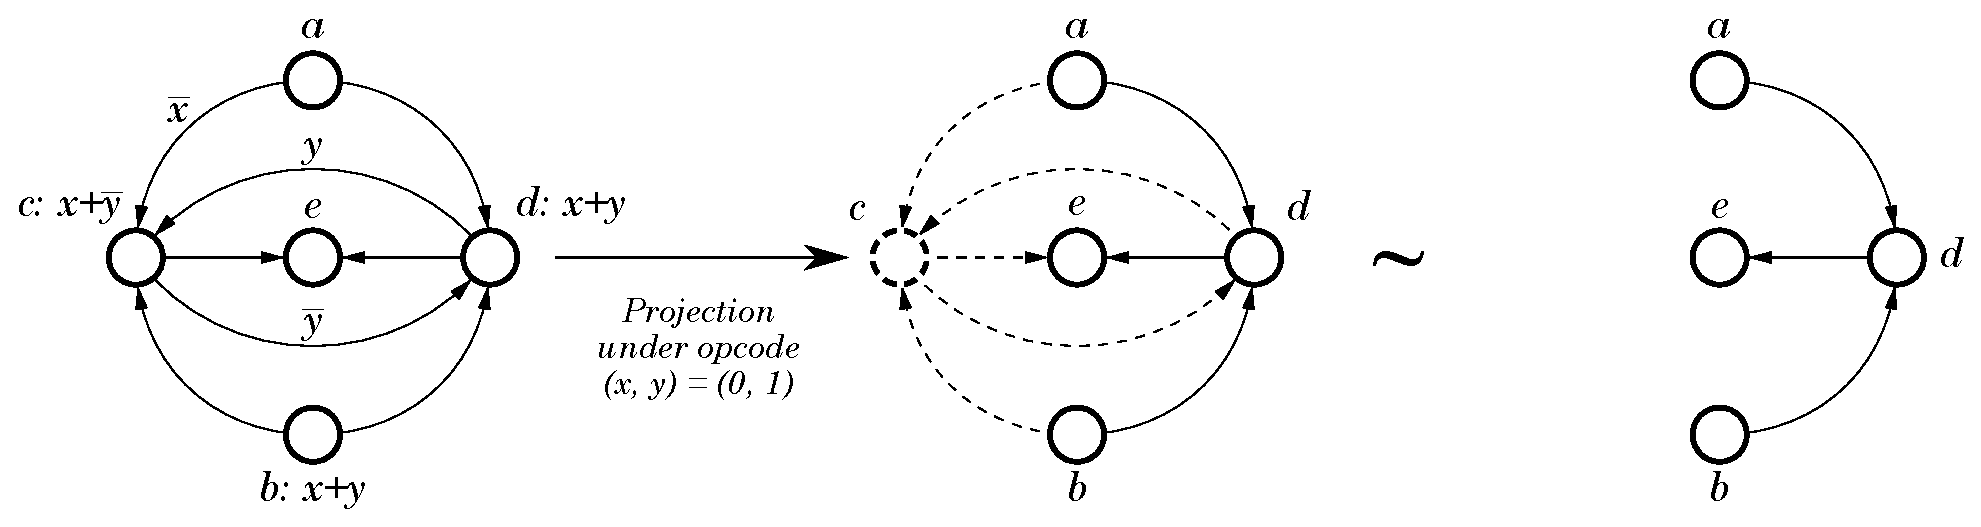
\includegraphics[scale=0.45]{fig/cpog_bin_2}}
\par\end{centering}

\begin{centering}
\subfloat[One-hot encoding (0001, 0010, 0100, 1000) and projection under opcode
0010]{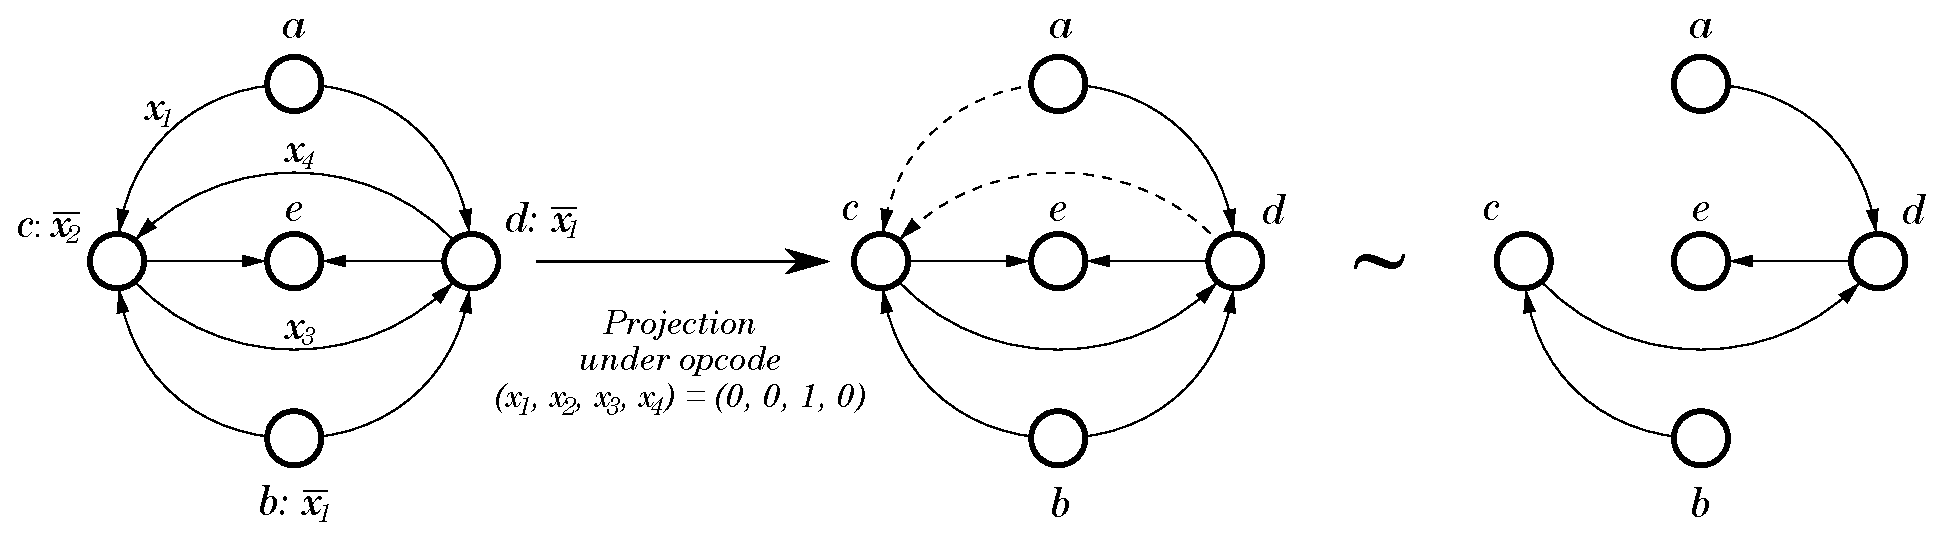
\includegraphics[scale=0.45]{fig/cpog_oh_2}}
\par\end{centering}

\centering{}\subfloat[Optimal encoding (010, 100, 111, 110) and projection under opcode
110]{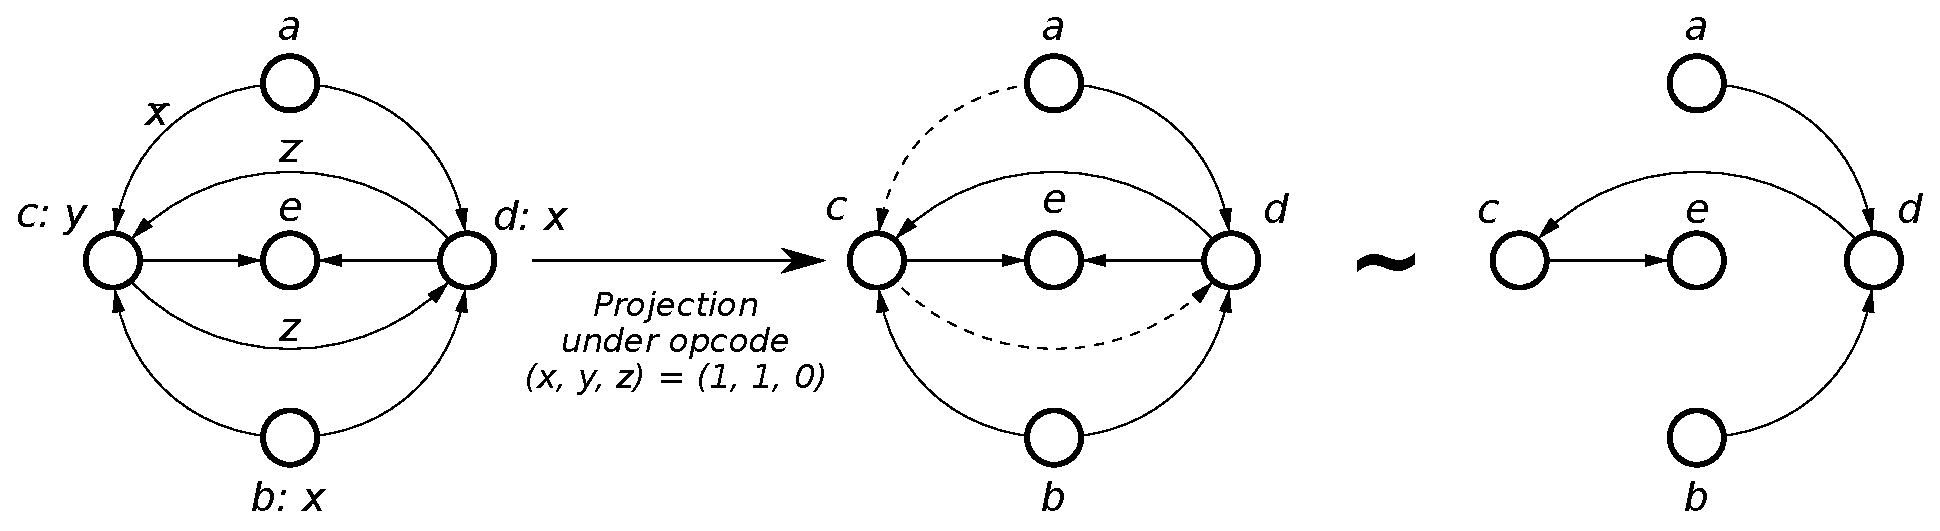
\includegraphics[scale=0.45]{fig/cpog_opt_2}}\caption{Different encoding schemes and projection examples\label{fig:Different-encoding-schemes}}
\end{figure}


\textbf{Binary encoding scheme}

This scheme uses the least possible number of variables $m=\left\lceil \log_{2}n\right\rceil $
to encode $n$ given partial orders. In our case two variables $X=\{x,\ y\}$
are used, and the opcodes are $\psi_{1}=(00)$, $\psi_{2}=(01)$,
$\psi_{3}=(10)$, and $\psi_{4}=(11)$. The synthesised CPOG and one
of its projections are shown in Figure~\ref{fig:Different-encoding-schemes}(a).
There are 9 literals in its vertex/arc conditions%
\footnote{Throughout the chapter we use operators `$+$' and `$\cdot$' to
denote Boolean disjunction (OR) and conjunction (AND), respectively.%
}.

\textbf{One-hot encoding scheme}

This is one of the most straightforward encoding schemes. It uses
$m=n$ variables to encode $n$ given partial orders such that $\psi_{k}[k]=1$
and $\psi_{k}[j]=0,\ j\neq k$. In our example, the four one-hot opcodes
are: $\psi_{1}=(1000)$, $\psi_{2}=(0100)$, $\psi_{3}=(0010)$, and
$\psi_{4}=(0001)$. Figure~\ref{fig:Different-encoding-schemes}(b)
shows the corresponding CPOG. Conditions on vertices $\{b,\ c,\ d\}$
became simpler; the total literal count was reduced to $6$. The price
for that is the increase in the number of variables from 2 to 4. Note
also that the projection under opcode $\psi_{3}=(0010)$ (shown to
the right) contains the transitive dependencies $b\rightarrow d$
and $c\rightarrow e$ which are not present in Figure~\ref{fig-Four-DAGs-specifying}(c).
Use of transitive dependencies helps to simplify arc conditions in
many cases (this and other optimisation techniques are discussed in~\cite{2010_mokhov_ieee}).

\textbf{Optimal encoding scheme}

It turns out that there is a middle-ground solution which uses the
same number of literals but only $3$ variables $X=\{x,\ y,\ z\}$.
The partial orders are encoded as $\psi_{1}=(010)$, $\psi_{2}=(100)$,
$\psi_{3}=(111)$ and $\psi_{4}=(110)$ leading to the CPOG in Figure~\ref{fig:Different-encoding-schemes}(c).
We call this encoding scheme optimal, because it is better than the
binary scheme (the resultant CPOG has fewer literals leading to a
simpler controller), and it is better than the one-hot scheme (it
uses fewer variables thus reducing the number of opcode wires coming
to the controller from the environment).

Given a CPOG $H$, there is a linear dependency between its complexity
$C(H)$, defined below, and the size of the synthesised controller~\cite{2010_mokhov_ieee}.
Figure~\ref{fig-Size-of-specification} shows a Pareto efficiency diagram comparing
different encoding schemes according to the number of variables they
use $|X|$ and complexity of the resultant CPOG. One can see that
the matrix encoding scheme~\cite{2009_mokhov_phd} produces CPOGs
with minimum possible size, but uses significantly more variables
than the binary one. We aim to reduce the number of used variables
but stay on the lower bound of CPOG complexity. In practice, the choice
of a particular encoding scheme is crucial. The resultant CPOGs (and
controllers) can differ in size by several orders of magnitude depending
on the chosen instruction codes. Now let us provide a formal definition
of CPOG optimality criteria.

\begin{figure}[h]
\begin{centering}
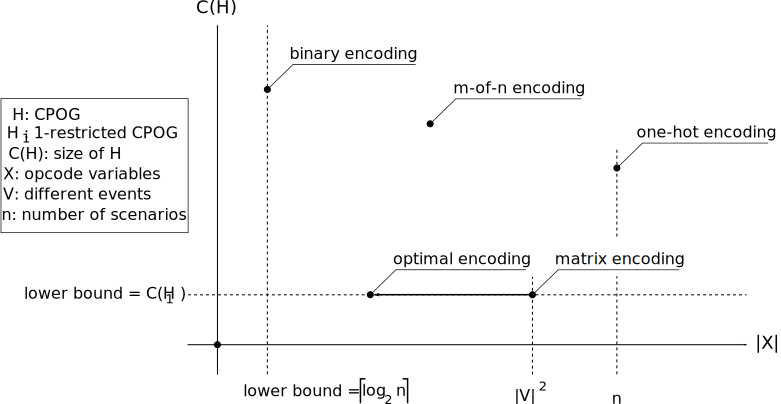
\includegraphics[width=0.75\columnwidth]{fig/encodings}

\par\end{centering}

\caption{Comparison of different encoding schemes\label{fig-Size-of-specification}}
\end{figure}

Complexity
of a CPOG $H$ is measured as a sum of literals in all of its vertex
and arc conditions $\phi$, i.e.
\[
C(H)\overset{\textrm{df}}{=}\sum_{v\in V}C(\phi(v))+\sum_{e\in E}C(\phi(e))
\]
A CPOG $H=(V,\ E,\ X,\ \rho,\ \phi)$ is called $k$-\emph{restricted}
iff its vertex and arc conditions $\phi$ are formulae having at most
$k$ literals, i.e. $\forall z\in V\cup E,\ C(\phi(z))\le k$. A \emph{$1$-}restricted
CPOG contains only formulae with single literals or constants as its
vertex and arc conditions. A $k$-restricted CPOG is called \emph{strongly $k$-restricted} 
iff there is a vertex or an arc with condition
having exactly $k$ literals, i.e. $\exists z\in V\cup E,\ C(\phi(z))=k$.

$C(H)$ strongly correlates with size and speed of the physical implementation
of a controller specified with $H$. Hence, we use $C(H)$ as an adequate
estimate of a CPOG $H$ efficiency. The following proposition states
that any optimal (w.r.t. measure $C$) CPOG is bound to be $1$-restricted.

\textbf{Proposition.} (Optimality) For any strongly $k$-restricted
($k>1$) CPOG $H$ there exists an equivalent%
\footnote{CPOGs are equivalent if they specify the same set of partial orders.%
} $1$-restricted CPOG $H_{1}$ such that $C(H_{1})<C(H)$.

Has been proven in \cite{2009_mokhov_phd}.

Although the above proof provides a polynomial algorithm for reduction
of any CPOG to a 1-restricted form, it is rather naive in terms of
the resultant size of variable set $X$. It adds as many new variables
as there are `heavy' ($C(\phi(z^{+}))>1$) conditions in the original
graph. In the worst case it uses $|V|^{2}$ additional variables which
can be impractical. The next subsection introduces a method which
uses the least possible number of variables to encode given partial
orders into a 1-restricted CPOG.


\subsection{Method for optimal encoding\label{sec:Method-for-optimal}
}

Let $\{P_{1},\ P_{2},\ \dots,\ P_{n}\}$ be a given set of $n$ partial
orders. The objective is to synthesise a $1$-restricted CPOG $H=(V,\ E,\ X,\ \rho,\ \phi)$
and to generate opcodes $\{\psi_{1},\ \psi_{2},\ \dots,\ \psi_{n}\}$
such that $H$ contains the given partial orders and the size of variable
set $X$ is minimised.

To solve this problem it is necessary to simultaneously satisfy all
the encoding constraints of graph $H$.

Formally, an \emph{encoding constraint} $\mathbf{e}(z)\in\{0,\ 1,\ -\}^{n}$
for a vertex or arc $z\in(V\cup E)$ is a vector of $n$ elements,
each corresponding to one of $n$ given partial orders. Element $\mathbf{e}(z)[k],\ 1\le k\le n$
is equal to $0$ iff condition $\phi(z)$ should evaluate to $0$
under opcode $\psi_{k}$ in order to produce correct partial order
$P_{k}$; $\mathbf{e}(z)[k]=1$ iff the condition should evaluate
to $1$; and $\mathbf{e}(z)[k]=-$ iff $\phi(z)$ can evaluate either
to $0$ or to $1$ (a \emph{don't care} value~\cite{1994_de_micheli_book},
as explained below).

\begin{table}[h]
\begin{centering}
\begin{tabular}{|c|c|c|c|c|c|c|}
\hline 
Vertices/arcs & \multicolumn{4}{c|}{Encoding constraint $\mathbf{e}(z)$} & \multicolumn{2}{c|}{Encoding $\phi(z)$}\tabularnewline
\cline{2-7} 
\multicolumn{1}{|c|}{$z\in V\cup E$} & $(-a)$ & $(a+b)$ & $(a-b)$ & $(-a-b)$ & \multicolumn{1}{c|}{pos. only} & \multicolumn{1}{c|}{pos./neg.}\tabularnewline
\hline 
\hline 
$a,\ e$ & $1$ & $1$ & $1$ & $1$ & $1$ & $1$\tabularnewline
\hline 
$a\rightarrow d$ & $-$ & $1$ & $1$ & $1$ & $1$ & $1$\tabularnewline
\hline 
$a\rightarrow e,\ b\rightarrow e$ & $-$ & $-$ & $-$ & $-$ & $0$ & $0$\tabularnewline
\hline 
$b\rightarrow c$ & $-$ & $-$ & $1$ & $-$ & $1$ & $1$\tabularnewline
\hline 
$b\rightarrow d$ & $-$ & $1$ & $-$ & $1$ & $1$ & $1$\tabularnewline
\hline 
$c\rightarrow e$ & $1$ & $-$ & $-$ & $1$ & $1$ & $1$\tabularnewline
\hline 
$d\rightarrow e$ & $-$ & $1$ & $1$ & $-$ & $1$ & $1$\tabularnewline
\hline 
\hline 
$b,\ d$ & $0$ & $1$ & $1$ & $1$ & $x$ & $x$\tabularnewline
\hline 
$c$ & $1$ & $0$ & $1$ & $1$ & $y$ & $y$\tabularnewline
\hline 
$a\rightarrow c$ & $1$ & $-$ & $0$ & $-$ & $z$ & $\overline{x}$\tabularnewline
\hline 
$c\rightarrow d$ & $-$ & $-$ & $1$ & $0$ & $w$ & $z$\tabularnewline
\hline 
$d\rightarrow c$ & $-$ & $-$ & $0$ & $1$ & $z$ & $\overline{z}$\tabularnewline
\hline 
\end{tabular}

\par\end{centering}

\caption{Encoding constraints\label{tab:Encoding-contstraints}}
\end{table}


Table~\ref{tab:Encoding-contstraints} shows all the encoding constraints
for partial orders in Figure~\ref{fig-Four-DAGs-specifying}. For
example, vertices $a$ and $e$ appear in all the four scenarios,
so $\mathbf{e}(a)=\mathbf{e}(e)=1111$ which means that $\phi(a)=\phi(e)=1$.
On the other hand, vertices $b$ and $d$ are not present in the first
scenario, and therefore their encoding constraint is $\mathbf{e}(b)=\mathbf{e}(d)=0111$.
First 11 rows of the table contain trivial\emph{ }encoding\emph{ }constraints,
i.e. constraints which do not contain $\mathbf{e}(z)[j]=0$ and $\mathbf{e}(z)[k]=1$
simultaneously ($j\neq k$). Vertices/arcs $z\in V\cup E$ with trivial
encoding constraints can be encoded with a Boolean constant ($\phi(z)=0$
or $\phi(z)=1$, see column `Encoding' in the table). Non-trivial\emph{
}encoding\emph{ }constraints (the last 5 rows of the table) cannot
be satisfied with a constant value, and therefore we need to introduce
operational variables to encode them, e.g. it is possible to satisfy
$\mathbf{e}(b)=\mathbf{e}(d)=0111$ with variable $x$: $\phi(b)=\phi(d)=x$.

Don't care values appear in a constraint in two cases:
\begin{itemize}
\item An arc $e=(v\rightarrow u)$ is not present in a partial order together
with one of its vertices. In this case $\phi(e)$ is allowed to evaluate
not only to $0$ but also to $1$, because if one of its vertices
is excluded from the partial order ($\phi(v)=0$ or $\phi(u)=0$)
then the arc is also excluded.
\item An arc $e=(v\rightarrow u)$ is transitive (i.e. $v\rightarrow t\rightarrow u$
for some $t\in V$). Therefore $\phi(e)$ is allowed to evaluate not
only to $1$ but also to $0$ (because transitive dependency $v\rightarrow t\rightarrow u$
is enough to guarantee $v\rightarrow u$ ordering).
\end{itemize}
Encoding constraint $\mathbf{e}(a\rightarrow c)=1\!-\!0-$ combines
these two cases. The first don't care is due to exclusion of vertex
$c$ in the second scenario ($\mathbf{e}(c)=1\underline{0}11$). And
the second don't care is due to transitive dependency $a\rightarrow d\rightarrow c$
in the fourth scenario ($\mathbf{e}(a\rightarrow d)=-11\underline{1}$
and $\mathbf{e}(d\rightarrow c)=-\!-0\underline{1}$).

Two encoding constraints $\mathbf{e}_{1}$ and $\mathbf{e}_{2}$ are
\emph{conflicting} iff
\[
\exists_{1\le k\le n},\ (\mathbf{e}_{1}[k]=1\wedge\mathbf{e}_{2}[k]=0)\vee(\mathbf{e}_{1}[k]=0\wedge\mathbf{e}_{2}[k]=1)
\]
In other words, it is impossible to find a Boolean vector satisfying
both constraints. For example, $\mathbf{e}(a\rightarrow c)=1\!-\!0-$
and $\mathbf{e}(c\rightarrow d)=-\!-\!10$ are conflicting, because
$\mathbf{e}(a\rightarrow c)[3]=0$ and $\mathbf{e}(c\rightarrow d)[3]=1$.
On the other hand, $\mathbf{e}(a\rightarrow c)=1\!-\!0-$ and $\mathbf{e}(d\rightarrow c)=-\!-\!01$
are not conflicting since vector $1001$ satisfies both of them. It
means that they can be resolved with the same variable (variable $z$
in Table~\ref{tab:Encoding-contstraints}, see column `Encoding:
pos. only').

The optimal encoding problem can now be formulated in terms of conflicting
encoding constraints: find an assignment of variables $\{x_{1},\ x_{2},\ \dots,\ x_{m}\}$
to constraints such that all pairs of the conflicting constraints
are assigned different variables and $m$ is minimised~\cite{2009_mokhov_phd}.
This problem belongs to the NP-complete complexity class and can be
reduced to the graph vertex colouring problem~\cite{2001_cormen_mit}:
a constraint must be `coloured' with a variable $x_{k}$ and any
two conflicting constraints must have different colours~\cite{2009_mokhov_phd}.

Figure~\ref{fig:Conflict-graph-colouring}(a) shows the conflict
graph for non-trivial encoding constraints from Table~\ref{tab:Encoding-contstraints}
and one of its optimal vertex colourings. It uses 4 `colours' $X=\{w,\ x,\ y,\ z\}$
and establishes the following encoding: $\psi_{1}=(0011)$, $\psi_{2}=(0100)$,
$\psi_{3}=(1110)$, and $\psi_{4}=(0111)$. This colouring is also
given in column `Encoding: pos. only' of the table. The synthesised
CPOG is shown in Figure~\ref{fig:Conflict-graph-colouring}(c); it
has the same size as the one-hot solution shown before but contains
only positive literals in its vertex/arc conditions.

Note that although encoding constraints $\mathbf{e}(c\rightarrow d)=-\!-\!01$
and $\mathbf{e}(d\rightarrow c)=-\!-\!10$ are conflicting they complement
each other. This opens another optimisation opportunity: it is possible
to resolve both constraints with a single variable $x$ using conditions
with complementary literals $x$ and $\overline{x}$, thus potentially
halving the number of used variables. In order to exploit this, we
build an \emph{extended conflict graph} which contains two vertices
for every encoding constraint $\mathbf{e}(z)$: one for the original
constraint and one for its inversion $\overline{\mathbf{e}}(z)$ which
is defined as
\[
\forall1\le k\le n,\ \overline{\mathbf{e}}(z)[k]=\begin{cases}
0 & \text{if }\mathbf{e}(z)[k]=1\\
1 & \text{if }\mathbf{e}(z)[k]=0\\
- & \text{if }\mathbf{e}(z)[k]=-
\end{cases}
\]
Exactly one vertex of every pair $\{\mathbf{e}(z),\ \overline{\mathbf{e}}(z)\}$
has to be coloured. If the vertex corresponding to an inverted constraint
$\overline{\mathbf{e}}(z)$ is chosen to be coloured with variable
$x$ it means that the constraint is resolved with negative condition
$\phi(z)=\overline{x}$. See Figure~\ref{fig:Conflict-graph-colouring}(b)
for the extended conflict graph of the example problem and its optimal
colouring. This colouring can also be found in column `Encoding:
pos./neg.' of Table~\ref{tab:Encoding-contstraints}. The synthesised
CPOG is shown in Figure~\ref{fig:Conflict-graph-colouring}(d) and
the generated opcodes of partial orders are $\psi_{1}=(010)$, $\psi_{2}=(100)$,
$\psi_{3}=(111)$ and $\psi_{4}=(110)$. This solution uses both positive
and negative literals for resolution of conflicting encoding constraints,
e.g. $\phi(c\rightarrow d)=z$ and $\phi(d\rightarrow c)=\overline{z}$,
resulting in only three operational variables $X=\{x,\ y,\ z\}$.
It is the optimal CPOG specification of the four partial orders from
Figure~\ref{fig-Four-DAGs-specifying}, there is no solution which
uses fewer literals.

The vertex colouring problem can be converted into an instance of
the Boolean satisfiability problem (SAT) for efficient solution as
explained in Section~\ref{sec:SAT-formulation}.

\begin{figure}[h]
\begin{centering}
\hfill{}\subfloat[Colouring with positive literals only]{\begin{centering}
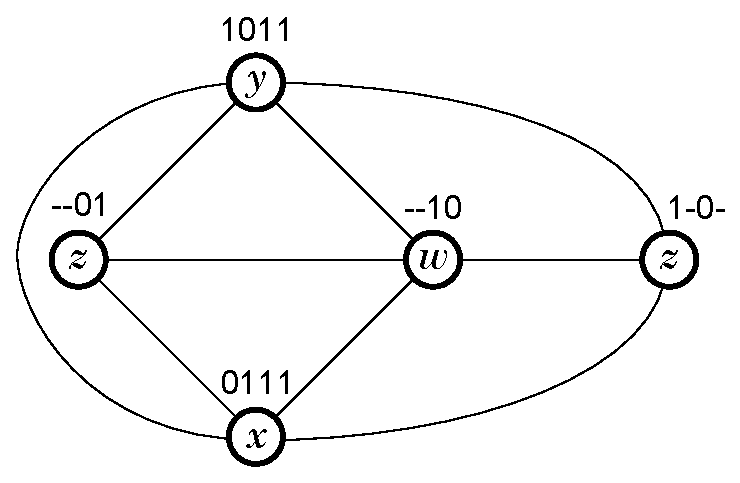
\includegraphics[bb=0bp 0bp 425bp 270bp,scale=0.45]{fig/conflict_graph_col}
\par\end{centering}

}\hfill{}\subfloat[Colouring with positive and negative literals]{\centering{}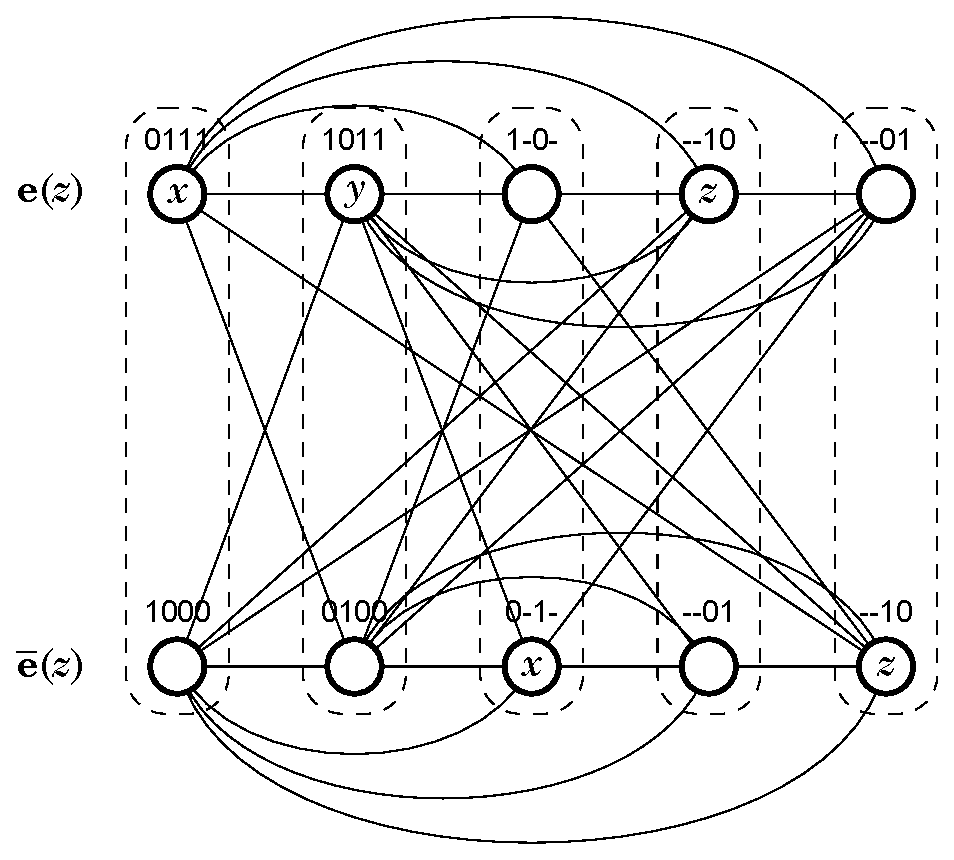
\includegraphics[scale=0.45]{fig/conflict_graph_inv}}\hfill{}
\par\end{centering}

\begin{centering}
\hfill{}\subfloat[CPOG with positive literals]{

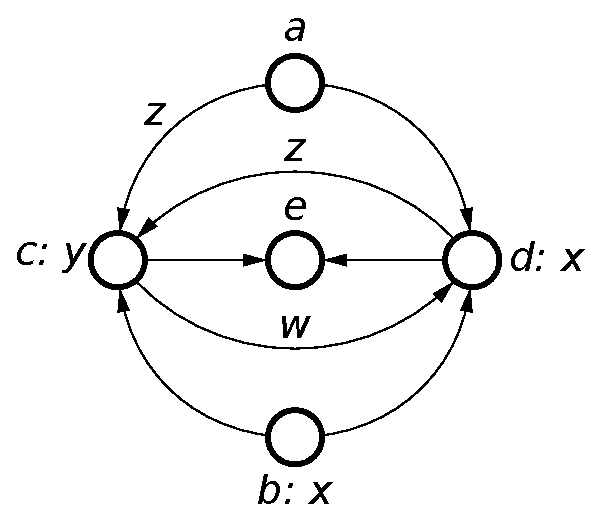
\includegraphics[scale=0.45]{fig/cpog_opt_woinv}}\hfill{}\subfloat[CPOG with positive and negative literals]{

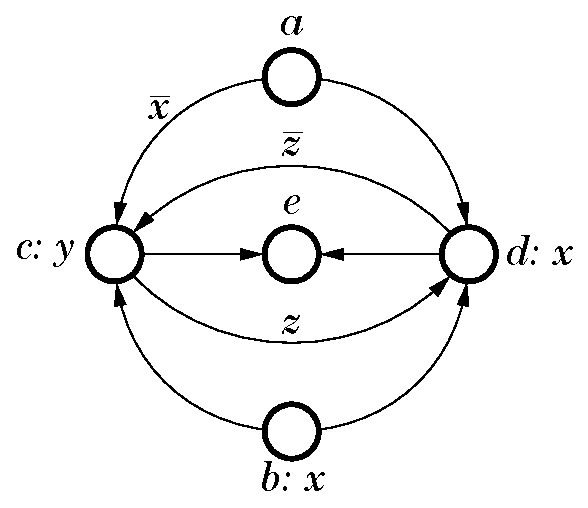
\includegraphics[scale=0.45]{fig/cpog_opt_w_inv}}\hfill{}
\par\end{centering}

\caption{Conflict graphs colouring and corresponding synthesised CPOGs\label{fig:Conflict-graph-colouring}}
\end{figure}




